\section{La creazione del server principale}

Il server principale è il componente con il compito di ricevere tutte le richieste dai client,
elaborarle e restituire le informazioni volute,
eventualmente a seguito di un'interrogazione verso la persistenza centrale.
Per poter essere in grado di rispondere a un numero sempre maggiore di utenti,
idealmente senza che questo impatti sul tempo di risposta o sulle performance in generale,
deve essere implementato in maniera tale da poter permettere un'esecuzione distribuita,
riducendo al minimo le dipendenze che possano minarne la duplicazione.\\
\\
Per soddisfare questo tipo di esigenza
esistono servizi definiti come Function as a Service (FaaS).
I FaaS sono servizi serverless,
ovvero la loro gestione hardware è completamente delegata al gestore del Cloud;
il cui scopo è quello di duplicare ed eseguire il progetto,
suddiviso e implementato attraverso molteplici Function.
Ogni Function consiste in un'unità indipendente di codice,
e in quanto tale crea la possibilità di essere eseguita in un ambiente di esecuzione unico per ogni richiesta.
Questa caratteristica, combinata con la virtualizzazione dell’ambiente di esecuzione,
consente una scalabilità potenzialmente illimitata.\\
\\
L’indipendenza della Function dipende dalla relazione con le altre parti del progetto e
dalla sua natura stateless.
L'esecuzione di una Function infatti,
oltre a dover essere limitata rispetto a qualunque dipendenza logica che possa dover essere condivisa,
deve essere svincolata dalle informazioni sullo stato o sulla sessione.
Queste caratteristiche, per loro natura, non possono essere garantite dal servizio,
e sono quindi una responsabilità di chi deve svilupparle.\\
\\
Per assicurarne l'autonomia,
le Function dovranno essere implementate seguendo il principio di singola responsabilità.
Ogni Function adempirà un solo compito specifico,
creando una restrizione delle dipendenze e
garantendo il minimo utilizzo di risorse necessarie per rispondere alla richiesta.
Inoltre, si semplifica così la creazione e la manutenzione del codice,
riducendo il controllo dell'esecuzione all'esito del tentativo di risoluzione del singolo problema.
\clearpage
\subsection{La scelta del servizio adatto}

I gestori in cloud che offrono servizi FaaS sono limitati.
Escludendo i fornitori improntati allo sviluppo di applicazioni principalmente front-end,
i fornitori sul mercato con servizi testati e maturi sono
Amazon Web Services con AWS Lambda, Azure con Azure Functions e Google Cloud Provider con Google Cloud Functions.
Tuttavia, queste tre soluzioni si assomigliano particolarmente.
Nonostante siano state tutte implementate usando una tecnologia proprietaria,
le proprietà computazionali, il supporto ai linguaggi e di costo risultano molto simili.\\
\\
Presentano tutti una granularità relativa alla scalabilità delle richieste a livello di funzione,
ovvero permettono di duplicare il solo codice necessario per l'esecuzione della funzione richiesta.
Il supporto ai linguaggi è molto esteso,
ma offrono tutti comunque la possibilità di implementare un runtime personalizzato,
di fatto supportando tutte le tecnologie.\\

\begin{longtable} {|P{3.5cm}|P{3.7cm}|P{3.7cm}|P{3.7cm}|}
    \hline
                                                    & \textbf{AWS Lambda}                                         & \textbf{Azure Functions} & \textbf{Google Cloud Functions} \\
    \hline
    \endhead
    Linguaggi supportati                            &
    Node.js, Python, Java, C\#, Go, PowerShell, Ruby, PHP
                                                    &
    Node.js, Python, Java, C\#, PowerShell, F\#, PHP
                                                    &
    Node.js, Python, Java, C\#, Go, F\#, Visual Basic                                                                                                                          \\
    \hline
    Runtime Personalizzato                          & Sì, tramite i custom deplyment packages o AWS Lambda Layers &
    Sì, grazie ai custom handlers                   &
    Sì, tramite immagini Docker personalizzate                                                                                                                                 \\
    \hline
    Massimo tempo di esecuzione                     &
    15 minuti                                       &
    Dai 10 ai 60 minuti, in base al piano di pagamento
                                                    &
    60 minuti per le richieste HTTP, 9 minuti per le richieste a eventi                                                                                                        \\
    \hline
    Massima memoria dedicata a funzione             &
    10 GB                                           &
    Da 1.5 GB a 14 GB in base al piano di pagamento &
    4 GB                                                                                                                                                                       \\
    \hline
    Tempo medio di attesa prima di essere spento    &
    Dai 5 ai 7 minuti                               &
    Tra i 20 e i 30 minuti                          &
    15 minuti                                                                                                                                                                  \\
    \hline
    Tempo medio di cold-startup                     &
    Generalmente sotto il secondo                   &
    Non oltre i 5 secondi                           &
    Da mezzo secondo a 2 secondi                                                                                                                                               \\
    \hline
    Orchestrazione                                  &
    Sì, tramite AWS Step Functions                  &
    Sì, tramite Durable Azure Functions             &
    Sì, tramite GCP workflow                                                                                                                                                   \\
    \hline
    \textbf{Costi}                                  &                                                             &                          &                                 \\
    \hline
    Richieste gratuite mensili                      &
    400.000 GB-seconds                              &
    400.000 GB-seconds                              &
    400.000 GB-seconds                                                                                                                                                         \\
    \hline
    Tempo di esecuzione gratuita al mese            &
    1 milione                                       &
    1 milione                                       &
    2 milioni                                                                                                                                                                  \\
    \hline
    Costo della richiesta al consumo                &
    \$0.20 per milione                              &
    \$0.20 per milione                              &
    \$0.40 per milione                                                                                                                                                         \\
    \hline
    Costo di esecuzione al consumo                  &
    \$0.000016 per GB-seconds                       &
    \$0.000016 per GB-seconds                       &
    \$0.0000125 per GB-seconds                                                                                                                                                 \\
    \hline
    Arrotondamento della durata                     &
    1 millisecondo                                  &
    1 millisecondo                                  &
    100 millisecondi                                                                                                                                                           \\
    \hline
    \caption{Caratteristiche delle principali FaaS}
\end{longtable}

La maggiore differenza tra queste soluzioni risulta nel tempo necessario in caso di start up,
ma va notato che, oltre a essere un caso particolare del funzionamento,
dipende molto dal linguaggio di programmazione,
dalle dipendenze e dalla dimensione del progetto.
Viene inoltre mitigato dal tempo di attesa prima di spegnere le istanze e
dalla quantità degli utenti attivi,
che, fornendo una continuità di richieste,
 contribuiscono a diminuire la frequenza dello spegnimento.\\
\\
Essendo le differenze tra un servizio e l'altro minime,
sia a livello di costi che di prestazioni,
ed essendo il progetto improntato su Azure,
la scelta della tecnologia su cui implementare il server principale è ricaduta sulle Azure Functions.\\

\subsection{Le scelte progettuali derivate dall'utilizzo delle Azure Functions}

L'utilizzo di un servizio FaaS comporta un approccio particolare per la scrittura del codice.
A differenza di un programma normale,
dove l'esecuzione del programma è indipendente dalla ricezione di un evento,
nelle FaaS l'invocazione di un processo avviene esplicitamente a partire da un fattore esterno
(che sia una richiesta HTTP o il messaggio in una coda).
Non bisogna più preoccuparsi di come far interagire le parti dell'applicazione,
ma piuttosto di come rispondere nella maniera più efficiente possibile a tanti particolari problemi.
Ogni funzione dovrà essere implementata come entità autonoma rispetto al resto del sistema,
con l'unica responsabilità di rispondere a un solo incarico specifico.\\
\begin{wrapfigure}{r}{0.25\textwidth}
    \centering
    
\includegraphics[height=.12\textheight]{functions.png}
    Azure Functions
\end{wrapfigure}
La difficoltà principale del procedimento sussiste nell'individuare i singoli compiti
in cui suddividere l'applicazione.
Raramente una richiesta può essere soddisfatta in un unico passaggio,
e non è quindi automatico che a una Function corrisponda una sola parte di codice,
soprattutto in quanto alcune richieste potrebbero avere alcune parti in comune
(ad esempio, l'autenticazione è necessaria alla maggior parte delle richieste).
Nel caso in cui una richiesta si componga di più passaggi logici,
per poterli racchiudere in un'unica Function bisogna analizzarne la relazione.\\
\par
Innanzi tutto ogni passaggio deve essere implementato sempre in maniera indipendente e stateless
come richiesto alle Function.
A questo punto è necessario però che tutti i passaggi siano in diretta successione,
e che il fallimento di uno solo di questi comporti il fallimento di tutta la funzione.
In caso contrario, è sconsigliato raggrupparle in un'unica Function,
quanto piuttosto suddividerli in altre piccole Function (con le stesse proprietà di cui sopra),
per poi coordinarle tramite l'utilizzo di un orchestratore o di code di eventi.\\
\\
L'orchestratore è una Function che ha la caratteristica
di poter invocare e controllare altre Function.
Consente di gestire efficacemente scenari
in cui è richiesta un'esecuzione particolare delle operazioni, sia essa sequenziale o parallela,
dove è necessario effettuare tentativi aggiuntivi in caso di errore o fallimento o
si richiede l'attesa del completamento di operazioni con un tempo di esecuzione prolungato.
Tuttavia, l'architettura stateless e l'accoppiamento debole tra orchestratore
e le Function in esecuzione causano un tempo di risposta delle richieste più elevato.\\
\\
Integrato all’interno delle Azure Functions,
Azure Durable Function consente la creazione di un orchestratore,
incaricato di gestire l’ordine, lo stato,
il ciclo di vita e le risposte delle varie Function coinvolte nell’elaborazione della richiesta,
mantenendo un'architettura indipendente e scalabile.\\
\\
Il coordinamento tramite code di eventi invece prevede,
durante l'esecuzione di una prima Function, l'invio di un evento al sistema.
L'evento verrà aggiunto in coda,
per poi invocare una seconda Function nel momento in cui sarà preso in carico.
Questo consente di separare logicamente le Function tra loro
senza introdurre ulteriori logiche e garantendo un tempo di risposta alla prima Function minimo,
ma introduce alcune problematiche.
Disaccoppiando le due Function la prima non ha conoscenza sull'esito della seconda,
ed è quindi necessario che la Function invocata dalla coda non svolga un compito essenziale
o che siano previste logiche di rilancio, controllo o segnalazione dell'esito.
Inoltre l'invocazione verrà così considerata come doppia, andando a influire sui costi totali.\\
\\
Come linguaggio di programmazione per lo sviluppo delle Function è stato utilizzato C\#.
La consapevolezza che sia l'ambiente di sviluppo di C\#,
ovvero il framework .Net, sia la piattaforma Azure
siano entrambi sviluppati e mantenuti dalla stessa azienda, Microsoft,
garantisce elevati livelli di stabilità, supporto e coordinamento delle tecnologie adottate.\\
\\
Azure Functions in ambiente .Net supporta due modelli di esecuzione e sviluppo:
in-process worker o isolated worker.
Il worker è il processo all’interno dell’applicativo che gestisce
la creazione delle risorse e l’esecuzione delle funzioni in risposta alle richieste.
Nella modalità in-process,
la funzione viene eseguita all’interno dello stesso processo del worker che l’ha generata,
riducendo la quantità di allocazione delle risorse necessarie
ma condividendo l’ambiente di esecuzione.
Nel modello isolated, invece,
ogni funzione viene eseguita creando un processo indipendente dedicato,
garantendo maggiore isolamento e quindi riducendo le possibili dipendenze tra le funzioni.\\
\\
Inoltre, il modello isolated worker offre ulteriori vantaggi grazie al maggiore supporto fornito:
innanzitutto esso prevede una maggiore compatibilità nel tempo,
grazie al più ampio numero di versioni del framework .Net a disposizione.
Il modello in-process, differentemente, è limitato alle sole versioni con supporto a lungo termine.
In secondo luogo il supporto per la creazione di middleware personalizzati
permette l'elaborazione di un codice intermedio tra la chiamata e l’esecuzione della funzione,
funzionalità invece non disponibile nel modello in-process.
Considerati questi vantaggi, le funzioni sono state sviluppate utilizzando il modello isolated worker
per garantire maggiore flessibilità, compatibilità e modularità dell’architettura.\\
\\
Lo sviluppo è stato condotto utilizzando Visual Studio Code,
programma sviluppato dalla stessa Microsoft per la creazione di codice.
Visual Studio Code permette l'integrazione con molteplici estensioni fornendo il supporto
per la maggior parte delle tecnologie.
In particolare, grazie alle estensioni dedicate al provider Azure,
è possibile collegare il proprio ambiente di lavoro con i servizi in cloud.
Il legame così creato consente un aggiornamento immediato e intuitivo del codice,
gestito interamente dal programma.\\
\\
\begin{figure}[h!]
    \begin{center}
        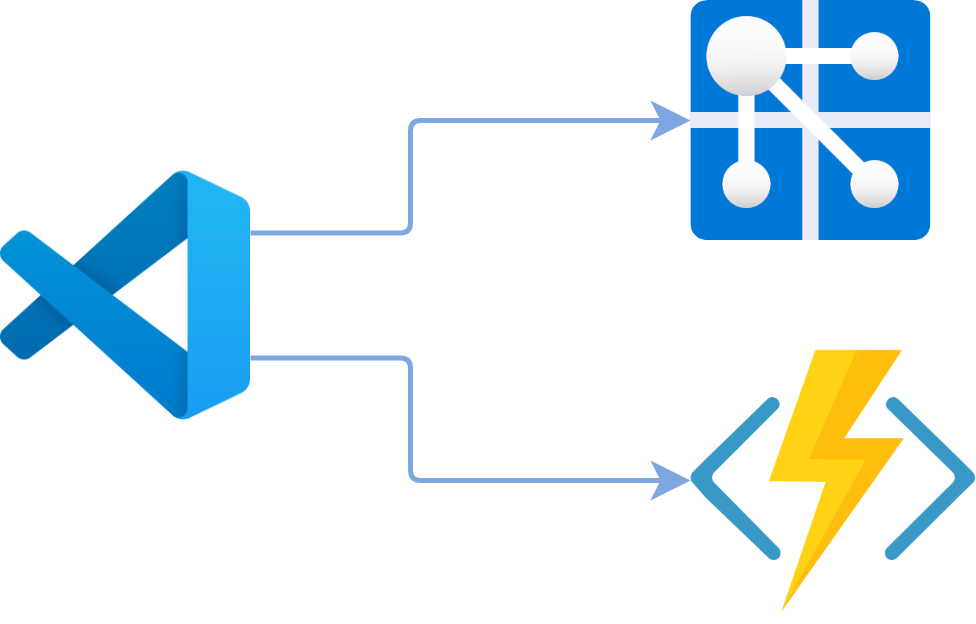
\includegraphics[height=0.10\textheight]{DeployBack.png}
        \caption{Diagramma di aggiornamento e distribuzione del server}
    \end{center}
\end{figure}

\clearpage


\subsection{L'implementazione della logica applicativa}
Per quanto ogni Function ricopra un unico compito,
alcune parti della sua risoluzione possono essere condivise con altre.
Per questo motivo,
la logica applicativa è stata suddivisa in metodi che risolvono una specifica esigenza logica,
che saranno poi inclusi nelle Function quando necessario.
I metodi vengono quindi raggruppati in classi in base all'inerenza dei loro scopi,
concentrando il codice che condivide le stesse necessità e uniformando il suo stile.
Le dipendenze vengono quindi inizializzate un'unica volta a livello di classe,
creando un software più ordinato.\\
\begin{figure}[h!]
    \begin{center}
        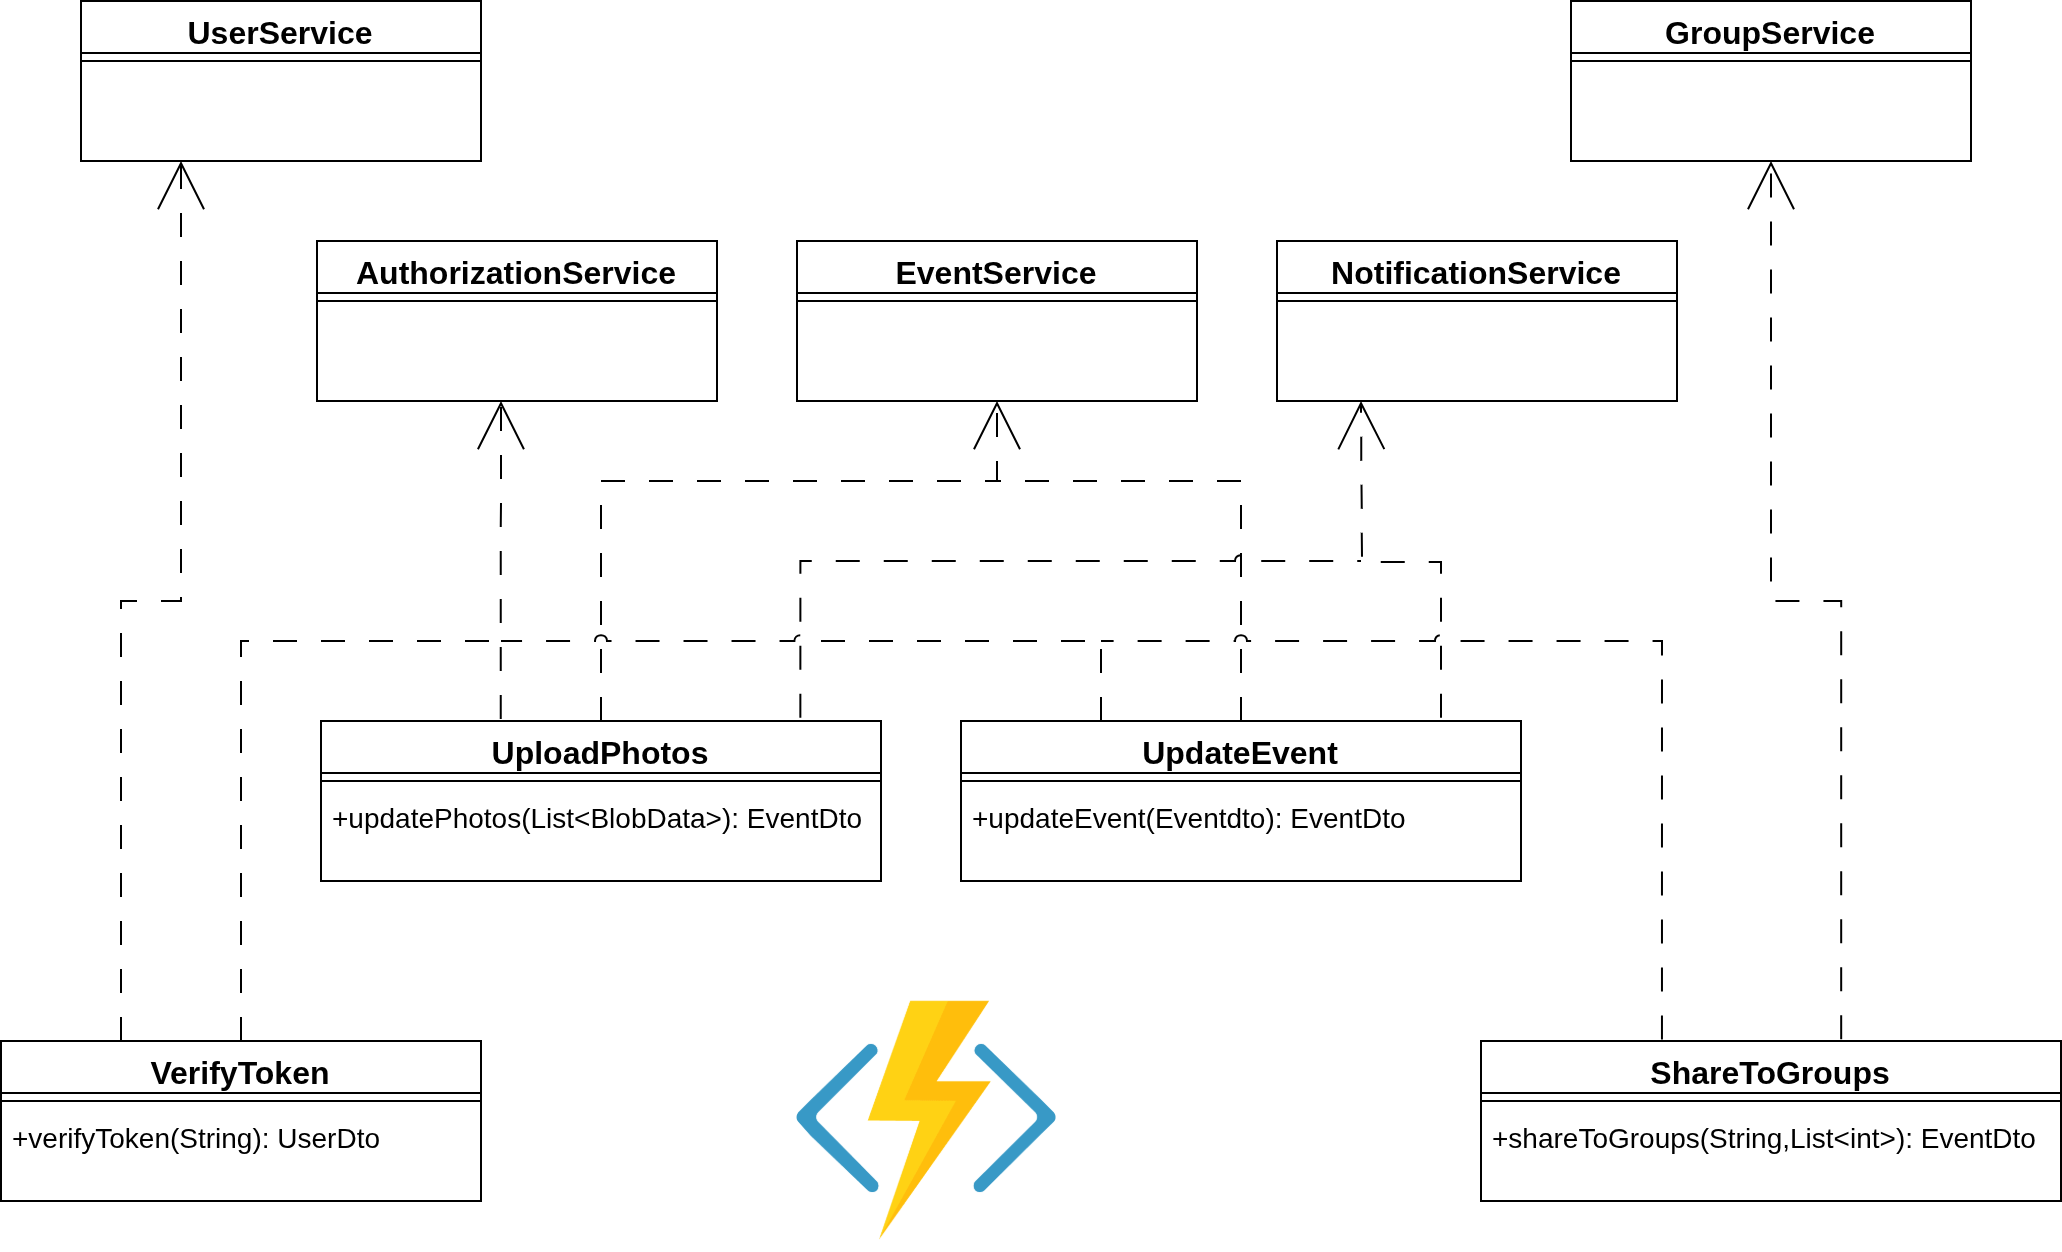
\includegraphics[width=\textwidth]{FunctionClassDiagram.png}
        \caption{Modello delle relazioni tra Functions e i servizi usati}
    \end{center}
\end{figure}

Con la stessa modalità di suddivisione delle responsabilità del client,
le classi sono state sviluppate tenendo conto delle divisioni del dominio
e di ulteriori responsabilità specifiche.
Per ogni elemento principale del dominio è stata sviluppata una classe service che implementa le operazioni relative,
mentre, per compiti che richiedono particolare attenzione o che astraggono l'interazione con una particolare risorsa,
vengono implementate classi apposite.\\
\clearpage


Ogni servizio relativo agli elementi strutturali ha bisogno di una connessione con il database
per poter applicare le modifiche eseguite.
Questa viene implementata da una classe chiamata WydDbService che racchiude la logica
e le impostazioni legate alla persistenza principale.
Si concentrano così in un unico luogo tutte le necessità e
le configurazioni di basso livello relative alla sua interazione,
quali la definizione del dominio e delle sue relazioni ed
eventuali operazioni da applicare in automatico qualora la natura dell'oggetto lo richieda.
L'implementazione delle classi del dominio viene trattata nei capitoli seguenti.\\

\begin{figure}[h!]
    \begin{center}
        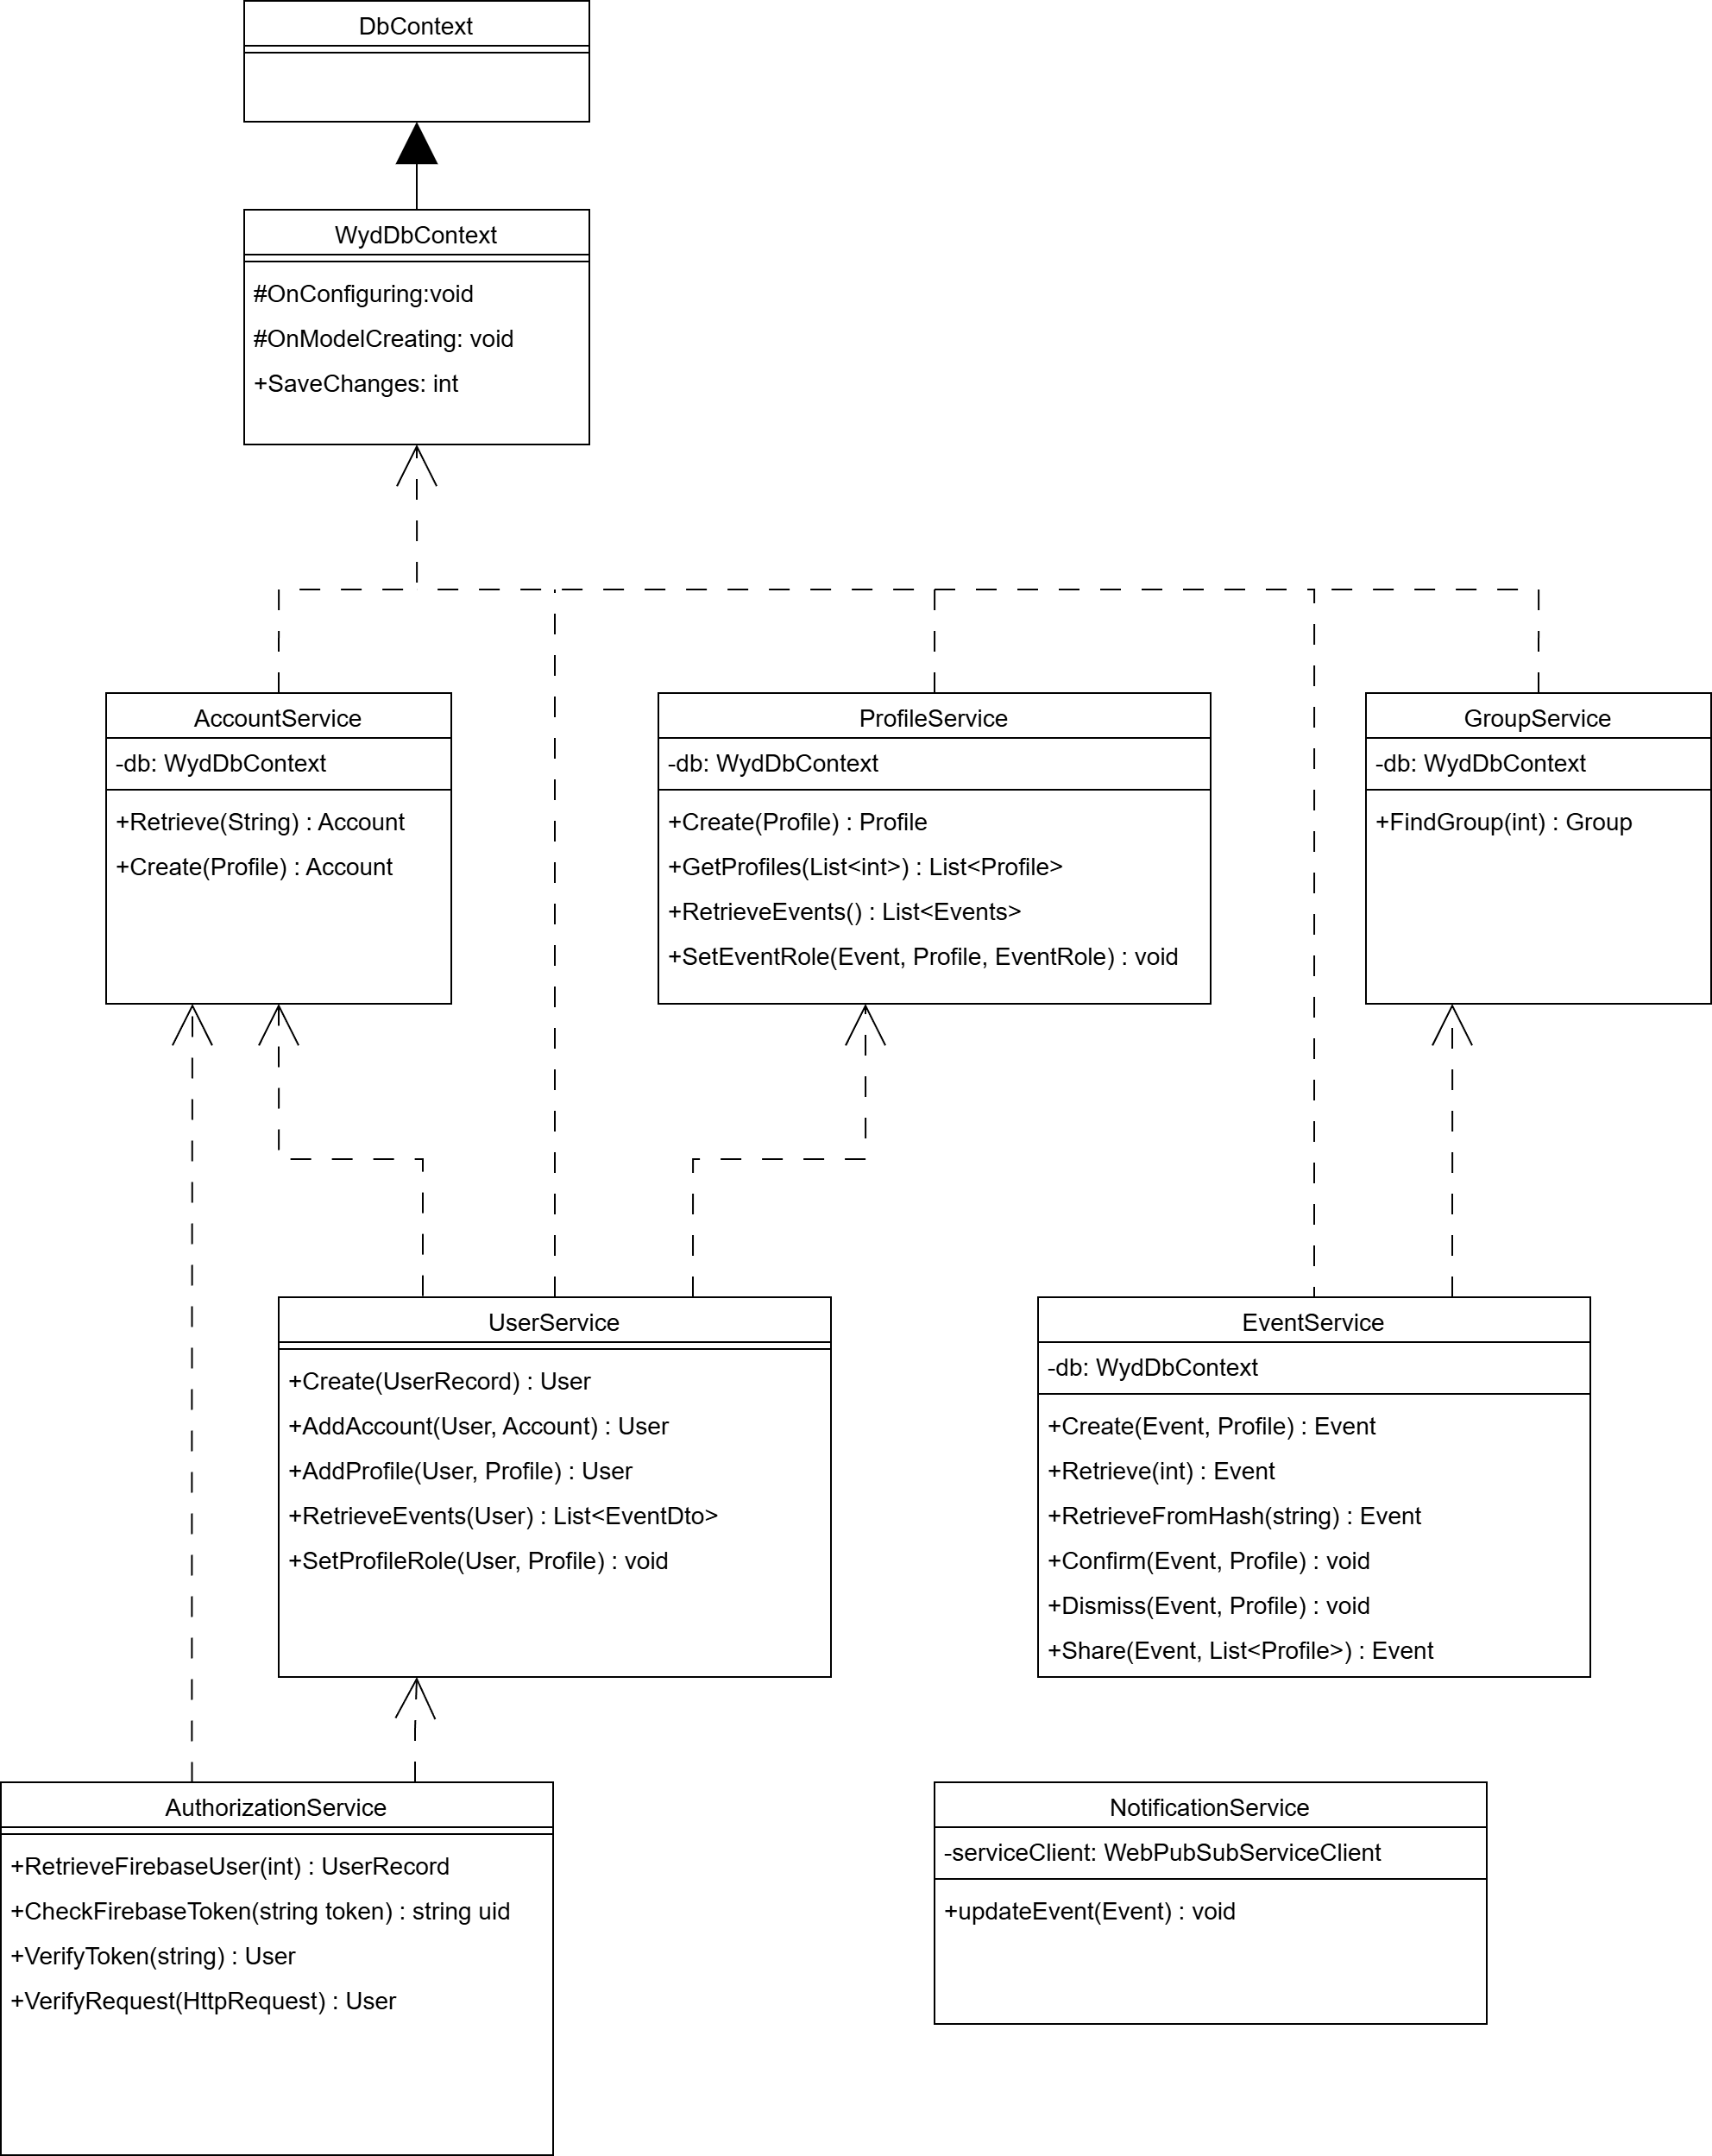
\includegraphics[height=0.8\textheight]{ServiceClassDiagram.png}
        \caption{Modello delle classi del server}
    \end{center}
\end{figure}
Per alcuni compiti specifici sono state implementate classi apposite.
In particolare, AuthorizationService si occupa dell'autenticazione e dell'autorizzazione della richiesta,
mentre NotificationService astrae la relazione con il servizio di aggiornamento in tempo reale.\\
\\
La maggior parte delle Function hanno il compito di rispondere a una richiesta REST,
in cui l'utente cerca di recuperare dei dati o di modificarli.
Ogni Function di questo tipo seguirà in generale lo stesso procedimento.
Il primo passo consiste nell'autenticare l'utente che fa la richiesta,
analizzando il relativo token.
Si controlla poi che l'utente abbia i permessi necessari per eseguire l'operazione desiderata.
Se è tutto in regola, si procede a elaborare i dati di ingresso, se necessario,
tramutandoli in oggetti logici.
Si esegue quindi l'azione voluta, la vera responsabilità della Function.
In base alla natura dell'operazione,
potrebbe essere opportuno inviare le notifiche degli aggiornamenti avvenuti.
Infine, si invia la risposta dell'operazione avvenuta a buon fine,
con in allegato i dati eventualmente necessari.
Tutto il processo viene inserito in un blocco che permette l'identificazione di errori e
la relativa risposta.\\
\\
Per allineare i dati a disposizione del server con il dominio del client
e per ridurre l'invio delle informazioni non necessarie, sono stati creati dei Data Transfer Object(DTO).
I DTO sono classi logiche che prevedono almeno un costruttore che, dato l'elemento del dominio,
ne copia solo le informazioni necessarie.
Questo permette di creare rappresentazioni dei dati come necessarie al client,
mascherando le logiche applicative e di fatto separando le dipendenze del dominio dai requisiti di comunicazione.\\
\\
\begin{figure}[h!]
    \begin{center}
        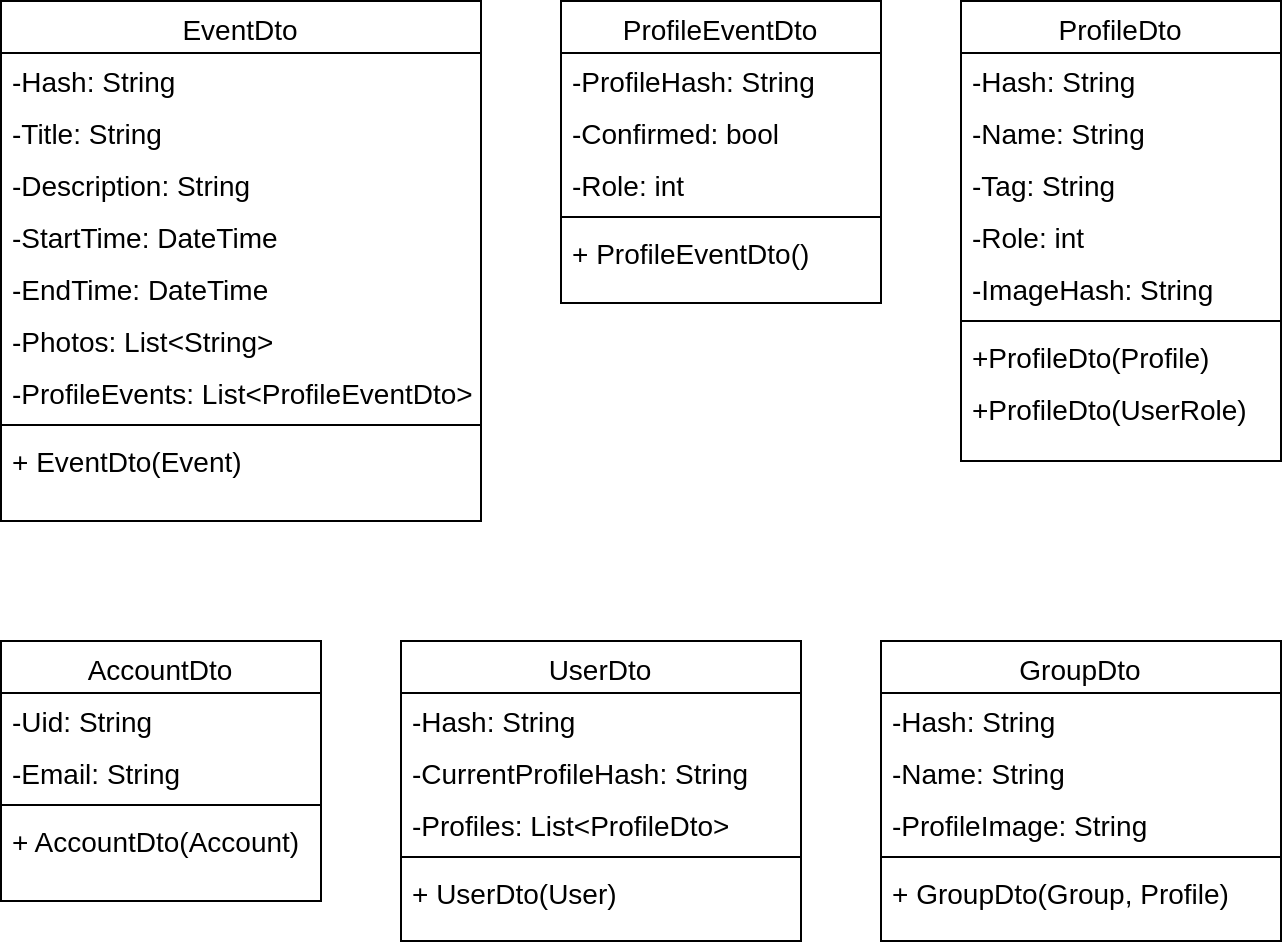
\includegraphics[width=\textwidth]{DTOClassDiagram.png}
        \caption{Modello delle classi dei data tranfer object}
    \end{center}
\end{figure}

Per ogni metodo pubblico delle classi service sono stati implementati dei test.
I test permettono la simulazione di differenti situazioni
per controllare che il codice segua il comportamento desiderato.
La loro implementazione è quindi precedente allo sviluppo stesso delle classi,
in quanto le aspettative sono già note, e il superamento dei test determina la correttezza del metodo.
Inoltre, in caso di necessità particolari che escono dalle normali aspettative della funzione,
quali, ad esempio, il controllo di un valore particolare o l'implementazione di un vincolo specifico,
i test assicurano la loro futura presa in carico anche in caso di modifica totale del codice.\\
\begin{figure}[h!]
    \begin{center}
        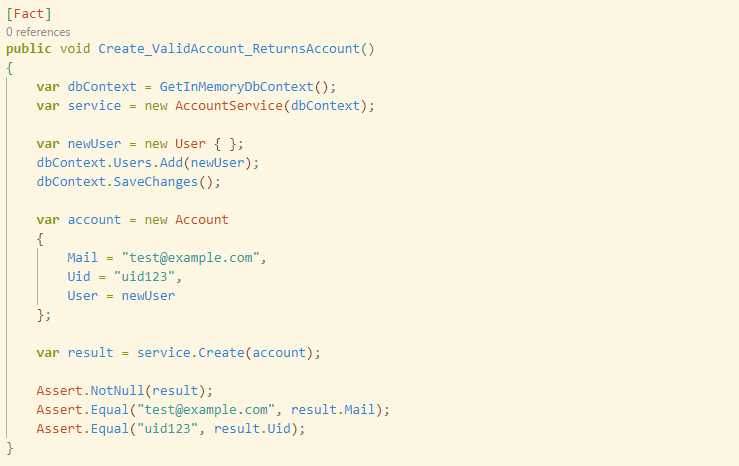
\includegraphics[height=.39\textheight]{TestAccount2.png}
        \caption{Test di creazione di un account}
    \end{center}
\end{figure}

\clearpage



